\documentclass[border=20pt]{standalone}
\usepackage{tikz}
\usepackage{xcolor}
\usetikzlibrary{positioning, arrows.meta, fit, backgrounds, calc}

%% ── Màu ──────────────────────────────────────────────────────────
\definecolor{cFront}{HTML}{6366F1}
\definecolor{cNginx}{HTML}{F59E0B}
\definecolor{cBack}{HTML}{10B981}
\definecolor{cAI}{HTML}{8B5CF6}
\definecolor{cPG}{HTML}{3B82F6}
\definecolor{cMG}{HTML}{16A34A}
\definecolor{cBg}{HTML}{F8FAFC}
\definecolor{cBorder}{HTML}{94A3B8}

%% ── Styles ───────────────────────────────────────────────────────
\tikzset{
  svc/.style 2 args={
    rectangle, rounded corners=7pt,
    minimum width=3.6cm, minimum height=1.3cm,
    align=center, font=\sffamily\bfseries\small,
    draw=#1!70, fill=#1!10, text=#1!80!black,
    line width=1.4pt
  },
  db/.style={
    rectangle, rounded corners=4pt,
    minimum width=2.8cm, minimum height=0.9cm,
    align=center, font=\sffamily\small,
    draw=#1!70, fill=#1!10, text=#1!80!black,
    line width=1.4pt
  },
  arr/.style={
    -Stealth, line width=1.1pt, color=#1!80
  },
  lbl/.style={
    font=\sffamily\scriptsize,
    fill=white, inner sep=2pt
  }
}

\begin{document}
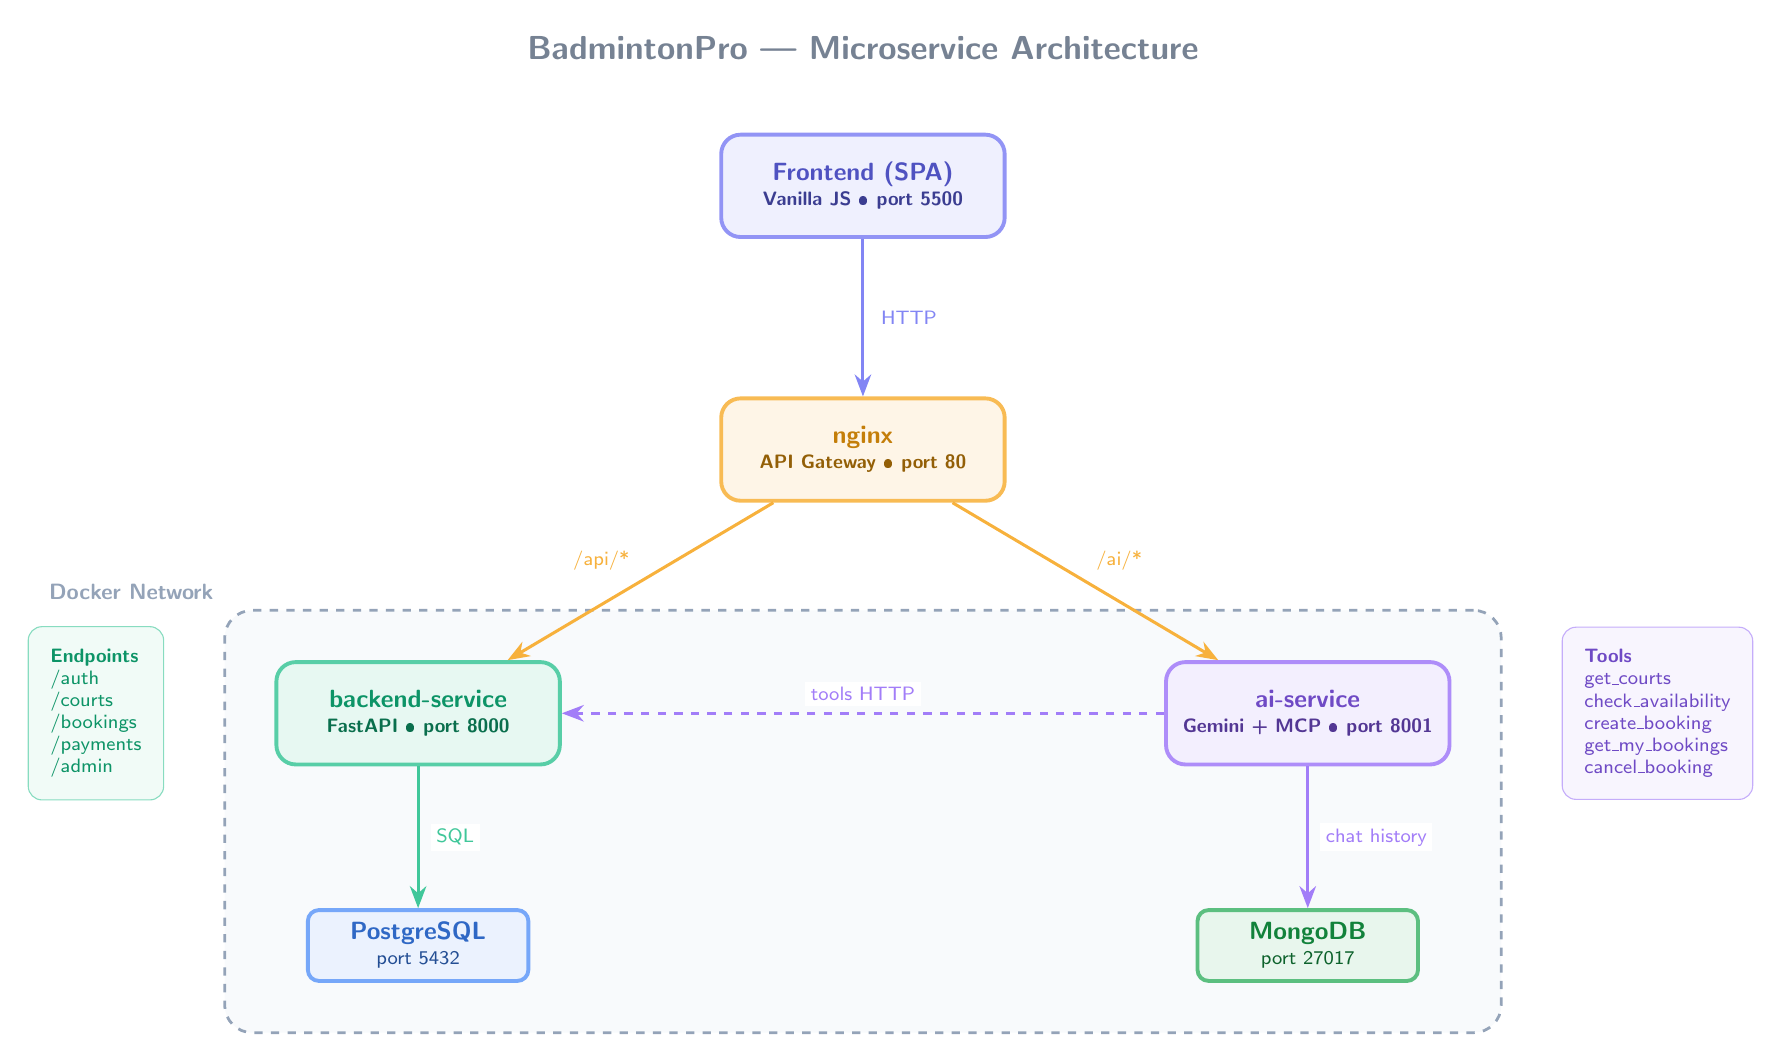
\begin{tikzpicture}[node distance=0pt]

%% ── Nodes ────────────────────────────────────────────────────────

% Frontend
\node[svc={cFront}{}] (fe) {
  \textcolor{cFront!80!black}{Frontend (SPA)}\\[-2pt]
  \textcolor{cFront!60!black}{\scriptsize\sffamily Vanilla JS \textbullet{} port 5500}
};

% nginx
\node[svc={cNginx}{}, below=2cm of fe] (nginx) {
  \textcolor{cNginx!80!black}{nginx}\\[-2pt]
  \textcolor{cNginx!60!black}{\scriptsize\sffamily API Gateway \textbullet{} port 80}
};

% backend
\node[svc={cBack}{}, below left=2cm and 2cm of nginx] (back) {
  \textcolor{cBack!80!black}{backend-service}\\[-2pt]
  \textcolor{cBack!60!black}{\scriptsize\sffamily FastAPI \textbullet{} port 8000}
};

% ai-service
\node[svc={cAI}{}, below right=2cm and 2cm of nginx] (ai) {
  \textcolor{cAI!80!black}{ai-service}\\[-2pt]
  \textcolor{cAI!60!black}{\scriptsize\sffamily Gemini + MCP \textbullet{} port 8001}
};

% PostgreSQL
\node[db={cPG}, below=1.8cm of back] (pg) {
  \textcolor{cPG!80!black}{\textbf{PostgreSQL}}\\[-2pt]
  \textcolor{cPG!60!black}{\scriptsize\sffamily port 5432}
};

% MongoDB
\node[db={cMG}, below=1.8cm of ai] (mg) {
  \textcolor{cMG!80!black}{\textbf{MongoDB}}\\[-2pt]
  \textcolor{cMG!60!black}{\scriptsize\sffamily port 27017}
};

%% ── Arrows ───────────────────────────────────────────────────────

% Frontend → nginx
\draw[arr=cFront] (fe) -- (nginx)
  node[lbl, midway, right=4pt] {\sffamily\scriptsize HTTP};

% nginx → backend
\draw[arr=cNginx] (nginx) -- (back)
  node[lbl, midway, above left=2pt] {\sffamily\scriptsize /api/*};

% nginx → ai
\draw[arr=cNginx] (nginx) -- (ai)
  node[lbl, midway, above right=2pt] {\sffamily\scriptsize /ai/*};

% ai → backend (internal tool calls, dashed)
\draw[arr=cAI, dashed]
  (ai.west) -- (back.east)
  node[lbl, midway, above=2pt] {\sffamily\scriptsize tools HTTP};

% backend → postgres
\draw[arr=cBack] (back) -- (pg)
  node[lbl, midway, right=4pt] {\sffamily\scriptsize SQL};

% ai → mongodb
\draw[arr=cAI] (ai) -- (mg)
  node[lbl, midway, right=4pt] {\sffamily\scriptsize chat history};

%% ── Sidebar: backend endpoints ───────────────────────────────────
\node[
  rectangle, rounded corners=5pt,
  draw=cBack!50, fill=cBack!6,
  align=left, font=\sffamily\scriptsize,
  text=cBack!80!black,
  left=1.4cm of back,
  inner sep=8pt
] {
  \textbf{Endpoints}\\
  /auth\\
  /courts\\
  /bookings\\
  /payments\\
  /admin
};

%% ── Sidebar: ai tools ────────────────────────────────────────────
\node[
  rectangle, rounded corners=5pt,
  draw=cAI!50, fill=cAI!6,
  align=left, font=\sffamily\scriptsize,
  text=cAI!80!black,
  right=1.4cm of ai,
  inner sep=8pt
] {
  \textbf{Tools}\\
  get\_courts\\
  check\_availability\\
  create\_booking\\
  get\_my\_bookings\\
  cancel\_booking
};

%% ── Docker network box ───────────────────────────────────────────
\begin{scope}[on background layer]
  \node[
    rectangle, rounded corners=10pt,
    draw=cBorder, fill=cBg,
    dashed, line width=1pt,
    fit=(back)(ai)(pg)(mg),
    inner sep=18pt,
    label={[font=\sffamily\footnotesize\bfseries, color=cBorder]
           north west:Docker Network}
  ] {};
\end{scope}

%% ── Tiêu đề ──────────────────────────────────────────────────────
\node[
  font=\sffamily\Large\bfseries,
  color=cBorder!80!black,
  above=0.8cm of fe
] {\large BadmintonPro — Microservice Architecture};

\end{tikzpicture}
\end{document}
